\chapter{Gomulscy z Anieliny, Wólki Mińskiej, Mikanowa i~Karoliny}

% Przednia okładka podrozdziału
\includepdf{Anielina_mapa_fin.png}

\section{Anielina: 1853~r. - 2024~r.}

Wieś Anielina została założona około 1820~roku w~odległości około dwóch 
kilometrów na południe od Mińska Mazowieckiego, na terenie ówczesnego 
Królestwa Polskiego. Anielina na początku swojego istnienia nosiła 
następujące nazwy w~księgach parafialnych: \enquote{Kolonia Anielin}, 
\enquote{Anielin} oraz \enquote{Angelin}, dopiero z~czasem utrwaliła 
się obecnie stosowana nazwa tej miejscowości. Wieś Anielina należała na 
początku XIX~wieku do parafii pod wezwaniem Narodzenia Najświętszej Maryi 
Panny w~Mińsku Mazowieckim. Najstarsza znana wzmianka Anielinie pochodzi 
z~1822~roku - jest to wpis w~aktach stanu cywilnego gminy Mińsk Mazowiecki, 
z~pierwszego lipca 1822~roku, dotyczący zgonu Marianny Zawadzkiej córki Jana 
Zawadzkiego i~Apolonii Kossakowskiej (patrz: ryc. \ref{fig:anielina_1822}). 
Zmarła wówczas Marianna Zawadzka urodziła sie niespełna klika miesięcy 
wcześniej w~sąsiedniej wsi Zakole\footnote{Co ciekawe Zawadzcy zamieszkujący 
wieś Anielina w~latach dwudziestych XIX~wieku to przodkowie Zawadzkich, 
którzy przeprowadzili się na przełomie XIX~i~XX~wieku do nowo powstałej 
wówczas wsi Desno - losy rodziny Zawadzkich spod Mińska Mazowieckiego zostaną 
szerzej omowione w~\hyperref[sec:zawadzcy]{załączniku numer IV}~do niniejszej 
książki.}. Poza wspomnianą rodziną Zawadzki, wieś Anielina na początku 
XIX~wieku zamieszkiwały również rodziny Sikorskich, Baranów Sadowskich czy 
Nalazków.

\begin{figure}[!ht]
    \vspace*{0.5cm}
    \centering 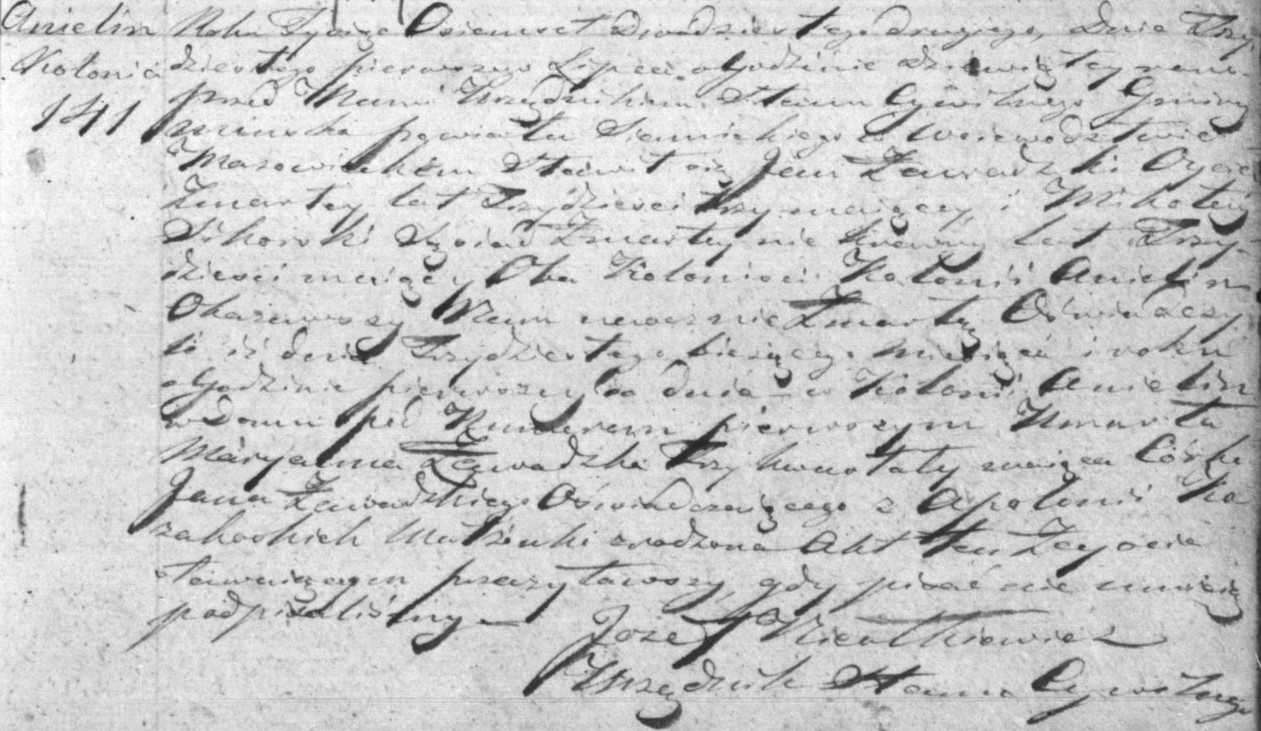
\includegraphics[width=1.0\linewidth]{
        Anielina_1822.jpg}
    \captionsetup{format=hang}
    \caption{Pierwszy znany wpis dotyczący wsi Anielina pochodzący 
    z~1822~roku z~akt stanu cywilnego gminy Mińsk Mazowiecki 
    \cite{par_minsk1}.}
    \label{fig:anielina_1822}
\end{figure}

% Przednia okładka podrozdziału
\includepdf{Wolka_Minska_mapa_fin.png}

\section{Wólka Mińska: 1861~r. - 2024~r.}

W~bieżącym

% Przednia okładka podrozdziału
\includepdf{Mikanow_mapa_fin.png}

\section{Mikanów: 1882~r. - 1894~r.}

W~bieżącym

% Przednia okładka podrozdziału
\includepdf{Karolina_mapa_fin.png}

\section{Karolina: 1896~r. - 2024~r.}

W~bieżącym
